
\section{Discussion}
\label{section:Discussion:Discussion}


This section presents the underlying discussion creating the basis for the model framework proposed in \Cref{section:Architecture}.
The discussion concerns the current state of time-series prediction, the motivation behind the method selection, model structure, and the selected error metric.
This section intendeds to answer the research questions proposed in this paper,
as well as the reason behind the framework.


\import{./sections/Conclusion/Discussion}{CurrentPredictions.tex}
\import{./sections/Conclusion/Discussion}{ProposedFramework.tex}
\import{./sections/Conclusion/Discussion}{ModelStructure.tex}
% \import{./sections/Conclusion/Discussion}{ErrorMetric.tex}

\section{Global versus Local models}
TODO:
% Write about which dataset the global model performs best on.
The global models seems to be doing be doing...

% Difference between MASE ans sMAPE
The global models seem to have a better 1 day MASE, but a lower sMAPE.
This is likely because sMAPE is not a symetric metric, as it punishes
under forcasts higher than over forecasts. Looking at the predictions made by
the local and global models, it seems that the global models in general tends to
under-forcast, and the local models has a tendency to over-forecast.

\section{LSTM trend and seasonality}
\begin{itemize}
  \item LSTM and ARIAM seem to have trouble with datasets with yearly seasonalities
  \item {LSTM will perform significantly better on these datasets if additional
        a multivariate version is used with additional information about date}
  \item {If date is not available then detrending the dataset using differencing is a good second alternative}
\end{itemize}


\section{Normalization versus Standardisation}
Our initial assumption was to use normalization to scale the data between a
fixed range between -1 and 1 because we did not know if the data would follow a Guassian
distribution. After testing both normalization and standardization,
standardization proved to perform significantly better.
The problem with scaling all values between a fixed range is that huge
outliers use up a lot of the range available, which will result in
most of the data having very small differences in values between them.
This can affect the NNs ability to differentiate between the observations.

\Cref{fig:time-series-standardization-vs-normalization} show two different time series
scaled with both techniques
\begin{figure}[h!]
  \centering
  \caption{Effects of different scaling techniques on a dataset with huge outliers.}
  \label{fig:time-series-standardization-vs-normalization}
  \begin{subfigure}[b]{0.49\textwidth}
    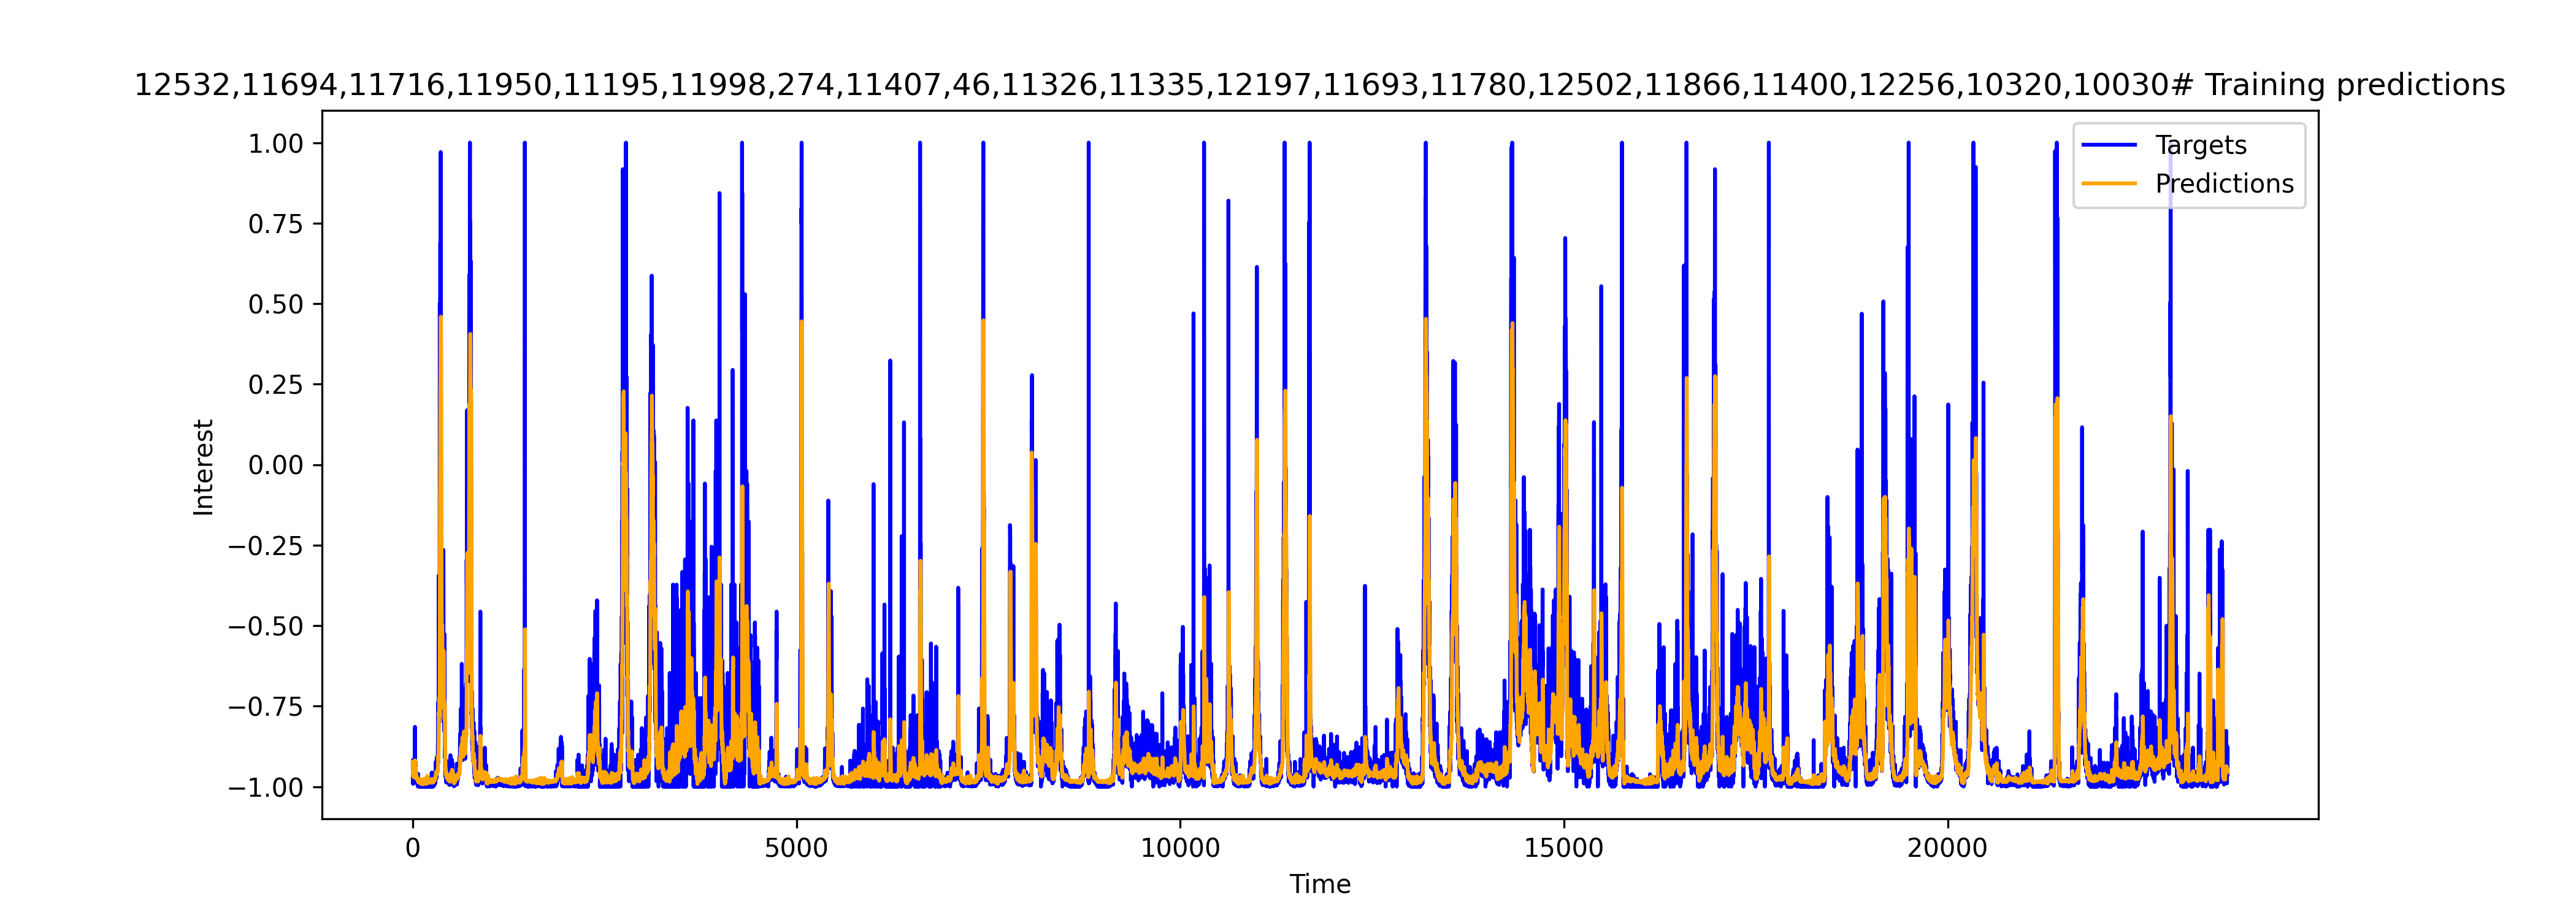
\includegraphics[width=\textwidth]{./figs/dataset/time-series_scaled_normalization2.png}
    \hfill
    \caption{A time series with huge outliers scaled using normalization. Most values are squeezed between -1 and -0.75.}
    \label{fig:time-series-normalization}
  \end{subfigure}
  \begin{subfigure}[b]{0.49\textwidth}
    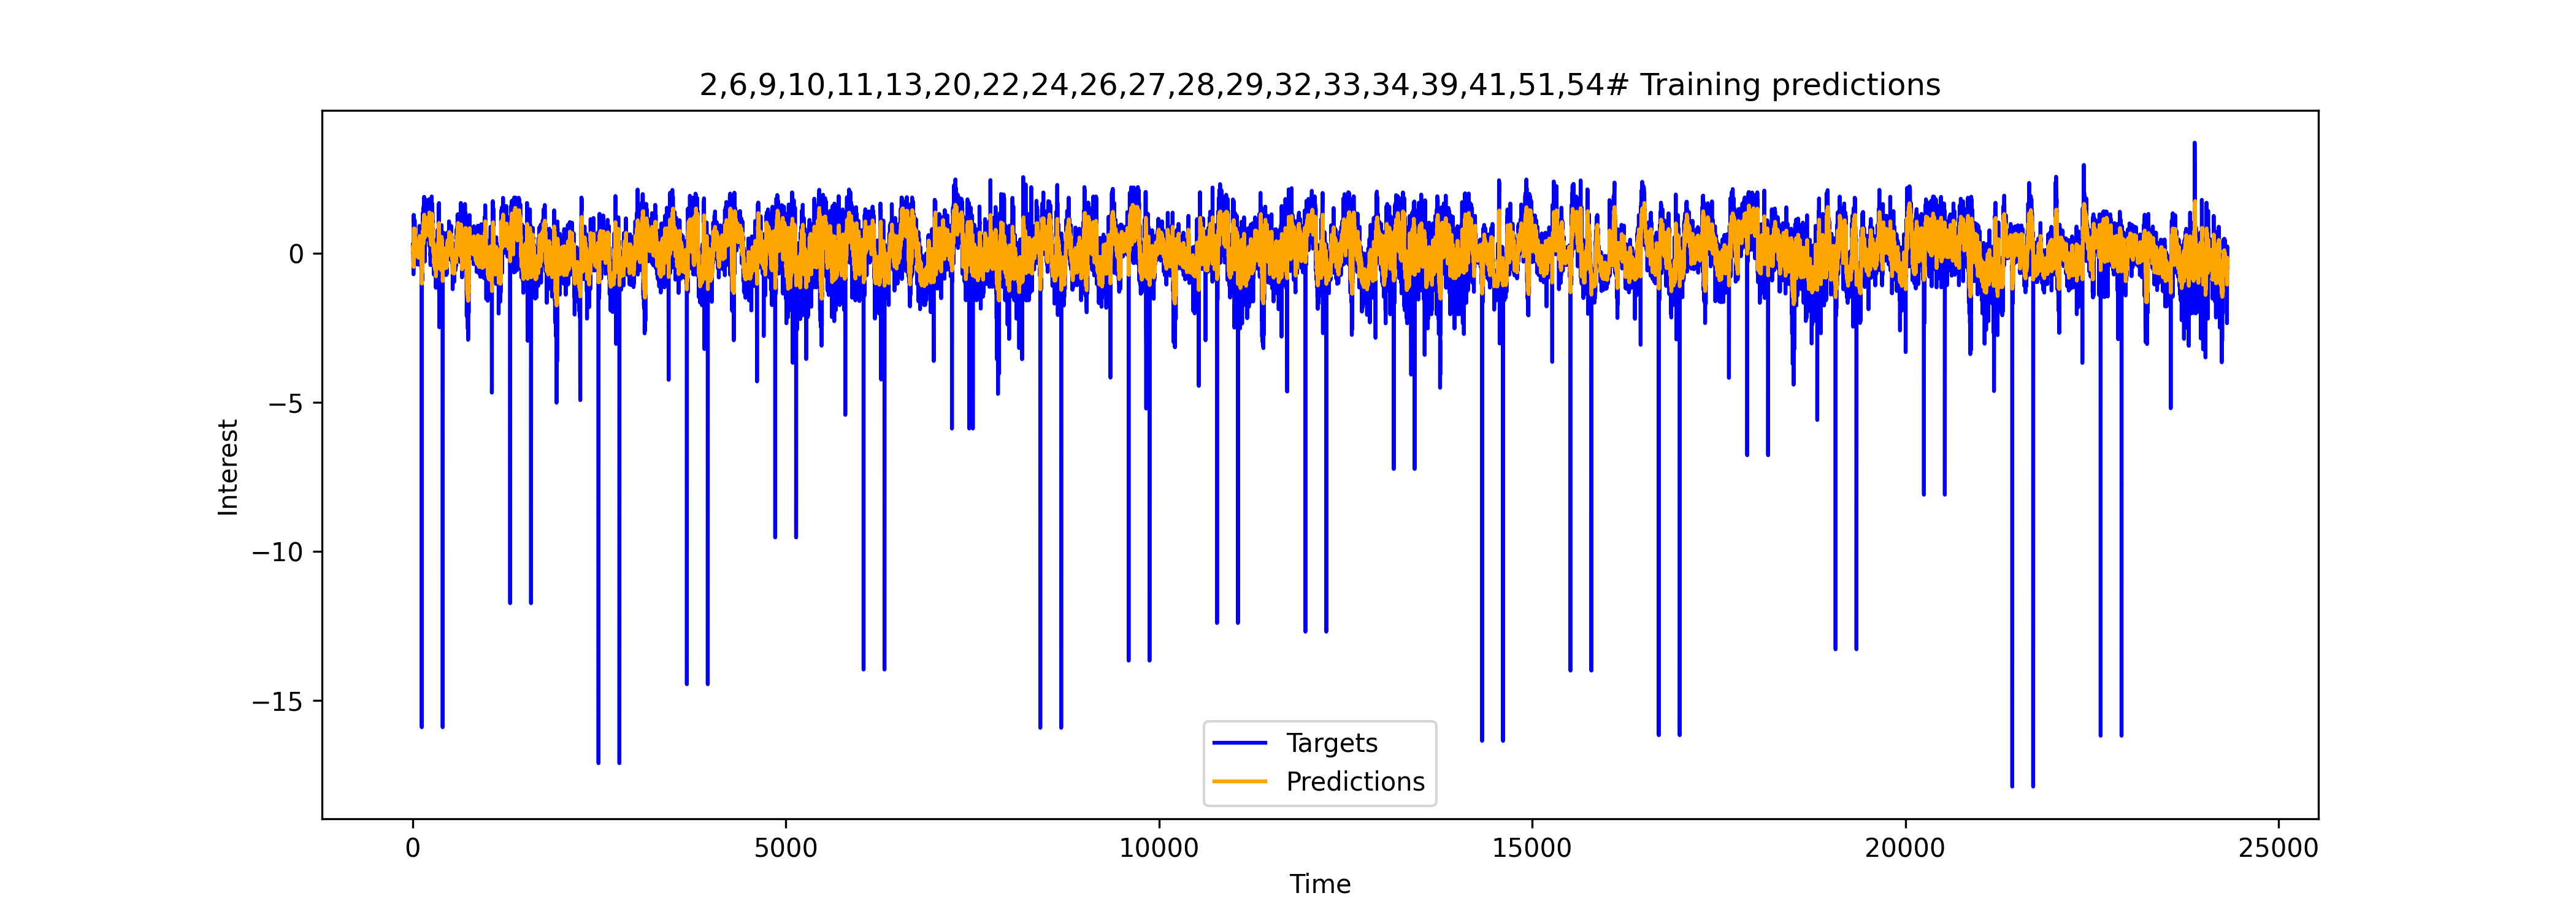
\includegraphics[width=\textwidth]{./figs/dataset/time-series_scaled_standardization.png}
    \hfill
    \caption{A time series scaled using standardization. Most values are centered between -2 and 2.}
    \label{fig:time-series-standardization}
  \end{subfigure}
\end{figure}

\section{Which datasets did we get poor results on and why?}
Do a lag scatter plot on datasets and compare them with datasets which got good results.